%% PIANO DI QUALIFICA

\section{Introduzione}
\subsection{Scopo del documento}


Lo scopo principale di questo documento è di ottenere una buona
qualità, intesa non solo come qualità di prodotto, ma anche come
qualità di processo. Per raggiungere tale obiettivo è necessario un
lavoro intellettuale e arduo poiché la qualità del software è diverso
dagli altri prodotti manifatturieri ed è difficile misurarla in
maniera oggettiva. Per rilevare e successivamente correggere le
anomalie in modo efficace è necessaria un'attività costante di
verifica e validazione da parte del \glossario{team} Obelix.


\subsection{Scopo del prodotto}

Lo scopo del prodotto è quello di creare un \glossario{SDK} che permetta la
realizzazione di cosiddette "bolle interattive" di diversi tipi in
base alle richieste di utenti (che nel nostro caso saranno gli
sviluppatori). Il prodotto si completerà con la realizzazione di una
demo presentabile mediante una web app con obiettivo di testare e
provare il corretto funzionamento del SDK.

\subsection{Glossario}
Al fine di evitare ogni ambiguità di linguaggio e massimizzare la
comprensione dei documenti, i termini tecnici, di dominio, gli
acronimi e le parole che necessitano di essere chiarite, sono
riportate nel documento \emph{Glossario vxxx}

\subsection{Riferimenti}

\subsubsection{Normativi}

\begin{itemize}
\item \textbf{Norme di progetto}:  \emph{Norme di Progetto vxxx}:
\item \textbf{Capitolato d'appalto C5}: \emph{RedBabel, Monolith \url{http://www.math.unipd.it/~tullio/IS-1/2016/Progetto/C5.pdf/}}

\end{itemize}

\subsubsection{Informativi}

\begin{itemize}
\item \textbf{Piano di Progetto}: \emph{Piano di Progetto}
\item \textbf{PDCA (Plan-Do-Check-Act): } \emph{\url{http://it.wikipedia.org/wiki/PCDA}}
\item \textbf{Standard ISO/IEC 12207:2008-IEEE Std 12207-2008}: \url{http://ieeexplore.ieee.org/xpl/mostRecentIssue.jsp?punumber=4475822}
\item \textbf{Standard ISO/IEC 15504}:  \url{http://en.wikipedia.org/wiki/ISO/IEC\_15504/}
\item \textbf{Standard ISO/IEC 9126}: \url{http://it.wikipedia.org/wiki/ISO/IEC\_9126}
\item \textbf{Indice di Gulpease}: \url{http://it.wikipedia.org/wiki/Indice\_Gulpease}
\end{itemize}



\section[Visione generale della qualità]{Visione generale della strategia di gestione della qualità}

% Con le strategie utilizzate si cerca di automatizzare il lavoro di
% verifica. Lo scopo è quello di ottenere un riscontro affidabile ed
% adeguato per assicurare un grado di qualità predeterminato e ridurre
% il lavoro manuale permettendo cosi una validazione semplificata.

%%%%%%%%%%%%%%%%%%%%%%%%%%%%%%%%%%%%%%%%%%%%%%%%%%%%%%%%%%%%%%%%%%%
%%%%%%%%%%%%%%%%%%%%%%%%%%%%%%%%%%%%%%%%%%%%%%%%%%%%%%%%%%%%%%%%%%%
%% RIFARE
%%%%%%%%%%%%%%%%%%%%%%%%%%%%%%%%%%%%%%%%%%%%%%%%%%%%%%%%%%%%%%%%%%%
%%%%%%%%%%%%%%%%%%%%%%%%%%%%%%%%%%%%%%%%%%%%%%%%%%%%%%%%%%%%%%%%%%%

\subsection{Obiettivi di qualità}

\subsubsection{Qualità di processo}
%% La qualità di processo è definita dallo standard ISO/IEC 15504
%% (SPICE). Questo standard specifica come la qualità è collegata alla
%% maturazione dei processi.
%% Non sarebbe possibile definire la qualità del prodotto senza garantire
%% la qualità del processo. La qualità del prodotto nasce dunque dalla
%% qualità del processo. Per garantire tutto ciò il team Obelix fa uso
%% dello standard ISO/IEC 15504 denominato SPICE, il quale fornisce gli
%% strumenti necessari a valutare l'idoneità dei processi.

La qualità di prodotto non può essere garantita a meno che non sia
garantita la qualità del processo che lo realizza. Nello standard
ISO/IEC 15504 (SPICE) viene definita la qualità di processo e vengono
fornite linee guida per la sua stima. Per maggiori informazioni sullo
standard si veda l'appendice A.1.
Adottando lo standard il gruppo Obelix sarà in grado di stimare
il livello di maturità raggiunto dal suo lavoro.

Nelle revisioni di progettazione il committente
fornisce una valutazione precisa del lavoro svolto fino a quel
momento.
Grazie a questo meccanismo e a valutazioni interne al gruppo è
possibile migliorare il metodo di lavoro.

\'E fondamentale inoltre rispettare i tempi stabiliti nel piano di
progetto vxxx. Per garantire una corretta stima è necessario misuare
eventuali discostamenti dalla pianificazione.

\paragraph{Miglioramento costante}

Tra una revisione di progettazione e la successiva è possibile
mettere a frutto quanto appreso nel periodo precedente.
Viene adottato il metodo manageriale PDCA (Plan,Do,Check,Act) che
permette l'uso di un approccio ingegneristico in un'attività generica.
In particolare si prescrive la misurazione di grandezze ritenute
rilevanti nello svolgimento delle attività al fine di averne una stima
oggettiva.
In seguito le informazioni così raccolte possono essere utilizzate per
individuare cambiamenti desiderabili nello svolgimento delle attività.
Per una descrizione più dettagliata del metodo PDCA si faccia
riferimento all'appendice \emph{B.1}


\paragraph{Rispetto della pianificazione}
Per capire se le attività di un processo sono in ritardo rispetto a
quanto pianificato all'interno del documento \emph{Piano di Progetto
  vxxx} viene utilizzata la metrica Schedule Variance. Si desidera che
il ritardo accumulato sia minore del 5\% rispetto al totale
pianificato. Sarebbe invece ottimale essere esattamente in linea con
quanto prevede il \emph{Piano di progetto vxxx}, o essere addirittura
in anticipo.

\paragraph{Rispetto del budget}
Viene utilizzata la metrica Budget Variance Per capire se i costi di
un processo rientrano nel budget previsto dal \emph{Piano di progetto
  vxxx}.
L’obiettivo minimo è quello di avere dei costi che non superano il
budget a disposizione per più del 10\%. Sarebbe invece ottimale che i
costi fossero esattamente in linea con il preventivo o addirittura
minori.

\subsubsection{Qualità di prodotto}
Lo svolgimento del progetto prevede la realizzazione di due prodotti:
i documenti e il software Monolith.
I documenti devono essere precisi e corretti nella forma e nei
contenuti in modo che possano essere un supporto efficace allo
svolgimento del lavoro.

Per garantire la qualità del software il team Obelix cercherà
di aderire al meglio allo standard di qualità ISO/IEC 9126 che
evidenzia quelli che possono essere gli aspetti rilevanti nella
valutazione della qualità di un software.

Per garantire la qualità del prodotto esistono i seguenti processi:
\begin{itemize}
\item \textbf{SQA: Software Quality Assurance} l'insieme delle
  attività realizzare al fine di garantire il raggiungimento degli
  obiettivi di qualità. \'E importante che tale processo sia
  preventivo e non correttivo
\item \textbf{Verifica} assicura che l'esecuzione delle attività dei
  processi svolti non introduca errori
  nel prodotto. Durante l'intera durata del progetto verranno svolte
  attività di verifica sugli
  output dei processi, accertando che esso sia corretto, completo e
  rispetti regole, convenzioni
  e procedure
\item \textbf{Validazione} la conferma oggettiva che assicura che i prodotti finali soddisfino i requisiti
  e le aspettative attese
\end{itemize}

\paragraph{Qualità dei documenti}
Gli obiettivi della qualità dei documenti che il team Obelix desidera raggiungere sono i seguenti:
\begin{itemize}
\item i documenti devono essere il più possibile comprensibili
\item i documenti devono essere corretti a livello ortografico
\item i documenti non devono contenere concetti errati
\end{itemize}

\subparagraph{Leggibilità e comprensibilità}
Per stimare la leggibilità e la comprensibilità dei documenti
viene utilizzato l’indice Gulpease. \'E desiderabile che i documenti
abbiano costantemente un indice maggiore
di 40 come soglia accettabile e 60 come ottimale. Per una descrizione
dettagliata della metrica utilizzata si faccia riferimento
alla metrica "Indice di Gulpease" alla sezione
\emph{2.8.2}. %%%%%%%%%%%%%%%%%%%%%%%%%%%%%%%%%%%%%%%%%%%%%%%%%%%%%%%%

\subparagraph{Correttezza ortografica}
Per capire quanto i documenti siano effettivamente corretti a livello
ortografico viene utilizzata la metrica "Percentuale di errori
ortografici rinvenuti e non corretti" . Si desidera che tutti gli
errori ortografici che sono stati trovati siano corretti. Per una
descrizione dettagliata della metrica utilizzata si faccia riferimento
alla metrica "Errori ortografici rinvenuti e non corretti" alla
sezione \emph{2.8.2}. %%%%%%%%%%%%%%%%%%%%%%%%%%%%%%%%%%%%%%%%%%%%%%%%%%%%%%%%%%%%%%%%%%%%%%%%%%5

\subparagraph{Correttezza concettuale}
Per capire quanto i documenti siano effettivamente corretti a livello
concettuale viene utilizzata la metrica "Percentuale di errori
concettuali rinvenuti e non corretti". L'obiettivo ottimale è quello
di correggere tutti gli errori trovati. Per una descrizione
dettagliata della metrica utilizzata si faccia riferimento alla
metrica "Errori concettuali rinvenuti e non corretti" alla sezione
\emph{2.8.2}.%%%%%%%%%%%%%%%%%%%%%%%%%%%%%%%%%%%%%%%%%%%%%%%%%%%%%%%%%%%%%%%%%%%%%%%%%%%%%%%%%%%%%%%%%%%


\paragraph{Qualità del software}

Al fine di garantire la qualità del prodotto software, il gruppo ha deciso di adottare lo standard
ISO/IEC 9126, esso classifica la qualità del software e definisce delle metriche utili alla sua
misurazione. In particolare il gruppo si prefigge di garantire le seguenti qualità per il prodotto
software:
\begin{itemize}
\item deve possedere le funzionalità descritte dai requisiti obbligatori
\item deve possedere le funzionalità descritte dai requisiti desiderabili
\item il codice deve risultare manutenibile e facilmente comprensibile
\item deve risultare affidabile e robusto
\item deve essere testato in ogni sua parte per garantirne il
  funzionamento
\end{itemize}
\subparagraph{Funzionalità obbligatorie}
Il prodotto deve implementare tutte le funzionalità descritte dai
requisiti obbligatori. Per monitorare lo stato di implementazione di
tali funzionalità si rapportano i requisiti obbligatori
completati con quelli ancora da completare. A tal fine viene
realizzato il tracciamento dei requisiti sui componenti
software\footnote{presente nlla Definizione di
  Prodotto vxxx}.
\subparagraph{Funzionalità desiderabili}
Il prodotto deve implementare la maggior parte possibile delle
funzionalità descritte dai requisiti desiderabili. Per monitorare lo
stato di implementazione di tali funzionalità si rapportano i
requisiti desiderabili
completati con quelli ancora da completare.
\subparagraph{Caratteristiche misurabili del software}
La qualità del software si misura attraverso l'adozione di metriche
scelte perchè ritenute rilevanti per descrivere le proprietà
critiche del software.
Oltre alle proprietà intrinseche del prodotto viene anche misurata la
qualità dei test, ovvero quanto i test effettivamente verifichino
l'assenza di anomalie nel software.
%%%%%%%%%%%%%%%%%%%%%%%%%%%%%%%%%%%%%%%%%%%%%%%%%%%%%%%%%%%%%%%%%%%%%%%%%%%%%%%%%%%%%%%%%%
%% da dire altro? ci deve essere una sezione dedicata? dove dire la
%% stategia di verifica?



%% \subsection{Procedure di controllo della qualità di processo}

%% Le linee guida per la gestione della qualità di processo seguono il
%% modello \glossario{PDCA} descrivendo come devono essere attuate le
%% procedure di controllo:

%% \begin{itemize}
%% \item Pianificazione dettagliata
%% \item Monitoraggio delle attività pianificate
%% \item Definizione delle risorse necessarie al conseguimento degli obiettivi
%% \item Utilizzo di metriche per verificare il miglioramento delle qualità dei processi
%% \end{itemize}

%% \subsection{Procedure di controllo della qualità di prodotto}

%% Con i seguenti processi verrà garantita il controllo della qualità del prodotto:
%% \begin{itemize}
%% \item \textbf{Software Quality Assurance (SQA)}: è l'insieme delle attività che serve per garantire il raggiungimento degli obiettivi di qualità
%% \item \textbf{Verifica}: assicura che non siano stati introdotti errori nel prodotto con l'esecuzione dei processi
%% \item  \textbf{Validazione}: è la conferma oggettiva che assicura che i prodotti finali soddisfino i requisiti e le aspettative attese
%% \end{itemize}

\subsection{Organizzazione temporale}

%Viene verificato la qualità dei singoli processi e dei loro output.

\subsubsection{Analisi}

In questo periodo verrà verificata la corrispondenza tra i casi d'uso
e i requisiti. Verrà inoltre controllato il rispetto dei processi e
della documentazione prodotta.

\subsubsection{Progettazione Architetturale}

In questo periodo avviene la verifica dei processi relativi all'analisi e
ai nuovi documenti di progettazione. Inoltre si verifica che i test
siano adeguatamente pianificati come descritti ed eseguiti nel documento \emph{Norme
  di Progetto vxxx}

\subsubsection{Progettazione di Dettaglio e Codifica}

In questo periodo avviene la verifica dei processi relativi alla
progettazione insieme alla verifica delle attività di codifica tramite
tecniche di analisi statica e dinamica.



\subsection{Tecniche di analisi}

\subsubsection{Analisi statica}
L’analisi statica è una tecnica di analisi che si applica sia alla
documentazione che al codice e permette di individuare errori ed
anomalie. Essa si può svolgere in due modi distinti che sono Walkthrough ed
Inspection.

\paragraph{Walkthrough}
\'E una tecnica che viene utilizzata soprattutto nelle prime attività
del progetto quando ancora non è presente una adeguata esperienza dei
membri del gruppo che permetta di attuare una verifica più
mirata e precisa.
Con l’utilizzo di questa tecnica, il \emph{Verificatore} sarà in grado
di stilare una lista di controllo con gli errori più frequenti in modo
da favorire il miglioramento di tale attività nel lavoro futuro.
Walkthrough è un’attività onerosa e collaborativa che richiede
l’intervento di più persone per essere efficace ed efficiente. Dopo
una prima fase di lettura e individuazione degli errori, segue una
fase di discussione con la finalità di esaminare i difetti riscontrati
e di proporre le dovute correzioni. L’ultima fase consiste nel
correggere gli errori rilevati e nello scrivere un rapporto che
elenchi le modifiche effettuate.


\paragraph{Inspection}
L’inspection consiste nell’analisi mirata di alcune parti dei
documenti o del codice ritenute maggior fonte di errore. Deve essere
seguita una lista di controllo per svolgere efficacemente questa
attività; tale lista deve essere redatta anticipatamente ed è
sostanzialmente frutto dell’esperienza maturata dai membri del team
con tecniche di walkthrough. L’inspection è dunque più rapida del
walkthrough, in quanto il prodotto viene analizzato solo in alcune
sue parti e con una lista di controllo ben precisa.

\subsubsection{Analisi dinamica}

L’analisi dinamica si applica solamente al prodotto software e viene
svolta durante l’esecuzione del codice mediante l’uso di test
progettati per rilevare la presenza di difetti.
L’obiettivo del test del software è infatti, quello di
realizzare un prodotto il più possibile esente da errori. Il
principale ostacolo alla fase di test è sintetizzato nella tesi di
Dijkstra, la quale afferma che il test può indicare la presenza di
errori, ma non ne può garantire l’assenza.
Affinchè tale attività sia utile e generi risultati attendibili è
necessario che i test effettuati siano ripetibili: dato un certo input
deve essere prodotto sempre uno stesso output in uno specifico
ambiente. Di conseguenza, i tre elementi fondamentali di un test sono:

\begin{itemize}
\item \textbf{Ambiente}: sistema hardware e software sui quali è stato
  pianificato l’utilizzo del prodotto software sviluppato. Su di essi
  deve essere specificato uno stato iniziale dal quale poter eseguire
  il test

\item \textbf{Specifica}: definizione di input e output
\item \textbf{Procedure}: definizione di come devono essere svolti i
  test, in che ordine devono essere eseguiti e come devono essere
  analizzati i risultati
\end{itemize}




%%%%%%%%%%%%%%%%%%%%%%%%%%%%%%%%%%%%%%%%%%%%%%%%%%%%%%%%%%%%%%%%%%%%%%%%%%%%%%%%%%%%%%%%%%%%%%%%%%%%
\section[Visione di dettaglio della qualità]{Strategia di gestione
  della qualità nel dettaglio}

Il Piano di Progetto vxxx fissa una serie di scadenze improrogabili e quindi risulta necessario definire
con chiarezza una strategia di qualifica efficace. Gli incrementi della documentazione o del codice
possono essere di natura programmata, quindi prefissati nel calendario, oppure possono insorgere
inaspettatamente. In questo caso sarà necessario programmare le dovute
modifiche.
La qualità di ogni incremento è basata sul rispetto delle Norme di
Progetto vxxx in quanto esse derivano da considerazioni di qualità.
Parte significativa del lavoro
verrà svolto con l’aiuto di automatismi che segnaleranno le problematiche rilevate in modo da
permettere una rapida correzione. L’utilizzo di software apposito permette di eseguire controlli
mirati minimizzando l'utilizzo di risorse umane. L’implementazione di tali controlli viene descritta nelle
Norme di Progetto vxxxx .



\subsection{Responsabilità}

La responsabilità delle verifiche è attribuita al  \emph{Responsabile di
  progetto} e ai  \emph{Verificatori} . All'interno del  \emph{Piano
  di Progetto vxxx}  sono definiti i compiti e le modalità di
attuazione.

\subsection{Risorse}
Il funzionamento del processo di verifica è garantito grazie al consumo di risorse, distinguibili
nelle categorie a seguire.
\subsubsection{Risorse umane}

Hanno maggiore responsabilità per l'attività di verifica
e validazione il \emph{Responsabile del progetto} e il
\emph{Verificatore}. Per una dettagliata descrizione dei ruoli e delle
loro responsabilità bisogna fare riferimento alle \emph{Norme di
  Progetto vxxx}. Per una dettagliata descrizione dell'impiego delle
risorse umane nell'arco del progetto bisogna riferimento al Piano di
progetto vxxx.

\subsubsection{Risorse tecnologiche}
Per risorse tecnologiche si intendono
tutti gli strumenti software e hardware che il gruppo Obelix intende
utilizzare per attuare le attività di verifica su processi e
prodotti. Per una dettagliata e accurata descrizione di tali strumenti
si faccia riferimento nelle \emph{Norme di Progetto vxxx}.



\subsection{Misure e metriche}
Con lo scopo di poter monitorare in modo consapevole l'andamento dei
processi e la qualità del prodotto si utilizzano delle metriche per
rendere misurabili e valutabili in modo oggettivo alcune
caratteristiche di documenti, processi e software.


\subsubsection{Metriche per i processi}
Le metriche per i processi hanno lo scopo  di monitorare e rendere
prevedibile l’andamento delle variabili di maggior criticità del
progetto: tempo e costo. Le metriche sono utilizzate in modo consultivo
per consentire un riscontro immediato sullo stato attuale del
progetto; ad ogni incremento verranno valutati tali indici e, se
necessario, verranno stabiliti opportuni provvedimenti da parte del  \emph{Responsabile di progetto}.

\paragraph{Schedule Variance}
Permette di calcolare le tempistiche rispetto l'organizzazione delle attività pianificate alla data
corrente. \'E un indicatore di efficacia soprattutto a beneficio del
cliente.
$$
SV = BCWP − BCWS
$$
Dove:
\begin{itemize}
\item \textbf{BCWP}: indica il valore delle attività realizzate alla data corrente
\item \textbf{BCWS}: indica il costo pianificato per realizzare le attività di progetto alla data corrente
\end{itemize}
Quindi con:
\begin{itemize}
\item $SV>0$: il lavoro prodotto è in anticipo rispetto quanto pianificato
\item $SV<0$: il lavoro è in ritardo
\item $SV=0$: il lavoro è in linea con quanto stabilito
\end{itemize}

\paragraph{Budget Variance}
Permette di calcolare i costi rispetto alla data corrente. \'E un indicatore che ha un valore
unicamente contabile e finanziario.
$$
BV = BCWS − ACWP
$$
Dove:
\begin{itemize}
\item \textbf{BCWS}: indica il costo pianificato per realizzare le attività di progetto alla data corrente
\item \textbf{ACWP}: indica il costo effettivamente sostenuto per realizzare le attività di progetto alla
  data corrente
\end{itemize}
Quindi:
\begin{itemize}
\item $BV>0$: il budget speso è minore di quanto pianificato
\item $BV<0$: il budget speso è maggiore di quanto pianificato
\item $BV=0$: il budget speso è in linea con quanto stabilito
\end{itemize}

\paragraph{Produttività}

\subparagraph{Produttività di documentazione}
Indica la produttività media nel redigere i documenti.
$$
\text{Produttività di documentazione} = \frac{\text{Parole}}{\text{Ore persona}}
$$
Dove:
\begin{itemize}
\item \textbf{Parole}: indica il numero di parole presente nei documenti
\item \textbf{Ore persona}: indica il numero di ore produttive impiegate per
  realizzare tali documenti
\end{itemize}

\subparagraph{Parametri utilizzati}
\begin{itemize}
\item Range-ottimale:$ [≥100]$
\end{itemize}

\subparagraph{Produttività di test}
Indica la produttività media nell'effettuare test.
$$
\text{Produttività di test} = \frac{\text{Numero di test}}{\text{Ore persona}}
$$
Dove:
\begin{itemize}
\item \textbf{Numero di test}: indica il numero di test eseguiti
\item  \textbf{Ore persona}: indica il numero di ore produttive
  impiegate per l'esecuzione di tali test
\end{itemize}

\subparagraph{Produttività di codifica}
Indica la produttività media nelle attività di codifica.
$$
\text{Produttività di codifica} = \frac{\text{LOCs}}{\text{Ore persona}}
$$
Dove:
\begin{itemize}
\item \textbf{LOCs}: indica il numero di linee di codice prodotte
  (Lines Of Code)
\item \textbf{Ore persona}: indica il numero di ore produttive
  impiegate per produrre tale codice
\end{itemize}

\paragraph{Copertura del test}
Indica la percentuale di casi coperti dai test eseguiti.
$$
\text{Copertura del test} = \frac{\text{Numero di funzioni testate} \times 100}{\text{Numero totale
    di funzioni disponibili}}
$$

\subparagraph{Parametri utilizzati}
\begin{itemize}
\item Range-accettazione: $[70 - 100]$
\item Range-ottimale: $[80 - 100]$
\end{itemize}






\subsubsection{Metriche per i prodotti}

\paragraph{Metriche per i documenti}
I documenti sono di qualità se sono leggibili. La leggibilità è
misurabile tramite un indice calcolabile sulle caratteristiche del
testo.

\subparagraph{Indice Gulpease}
L'indice Gulpease misura la leggibilità di un testo in Italiano
utilizzando variabili linguistiche come la lunghezza delle parole e
delle frasi.

$$
G = 89 + \frac{300 \times \text{numero delle frasi} - 10 \times \text{numero delle lettere}}{\text{numero
    delle parole}}
$$

Il valore risultante è un numero compreso tra 0 e 100, dove 100 indica
la
leggibilità massima e 0 la leggibilità minima. I documenti sono da
considerare secondo le seguenti fasce:
\begin{itemize}
\item $ G < 80 $ sono considerati difficili per chi ha la sola licenza
  elementare
\item $ G < 60 $ sono considerati difficili per chi ha la sola licenza
  media
\item $ G < 40 $ sono considerati difficili per chi ha un diploma di
  scuola  superiore
\end{itemize}

\textbf{Parametri utilizzati}\\
\begin{itemize}
\item Range di accettazione [40-90]
\item Range ottimale [50-90]
\end{itemize}

\subparagraph{Errori ortografici rinvenuti e non corretti}
Questa metrica è necessaria per capire quanto un documento sia
corretto dal punto di vista ortografico. Gli strumenti automatici
possono trovare la maggior parte degli errori ortografici all'interno
di un testo ma non sono molto attendibili poichè si basano sul numero
degli errori rinvenuti ma non successivamente corretti. Vengono di
seguito riportati i range stabiliti per quest'ultima metrica:
\begin{itemize}
\item una percentuale di errori non corretti maggiore allo 0\% è ritenuta negativa
\item una percentuale di errori non corretti pari allo 0\% è ritenuta accettabile
\item una percentuale di errori non corretti minore allo 0\% è ritenuta ottimale
\end{itemize}

\subparagraph{Errori concettuali rinvenuti e non corretti}
Questa metrica è necessaria per capire quanto un documento sia
corretto dal punto di vista concettuale. Vengono di seguito i range
stabiliti per la metrica appena introdotta:
\begin{itemize}
\item una percentuale di errori non corretti maggiore al 5\% è ritenuta negativa
\item una percentuale di errori non corretti minore del 5\% è ritenuta accettabile
\item una percentuale di errori non corretti pari allo 0\% è ritenuta ottimale
\end{itemize}





\paragraph{Metriche per software}
%%%%%%%%%%%%%%%%%%%%%%%%%%%%%%%% INTRO
Di seguito vengono elencate le metriche per il software prodotto e le relative caratteristiche di
qualità che intendono valutare.

\begin{center}

  \begin{tabular}{|l|c|}
   % {|>{\centering}m{6cm} ||>{\centering}m{6cm}|}
    \hline
    \textbf{Metriche scelte} & \textbf{Caratteristiche di qualità} \\
    \hline
    %Copertura requisiti obbligatori  & Funzionalità \\
    %Copertura requisiti desiderabili & Funzionalità \\
    Complessità ciclomatica  & Manutenibilità \\
    Numero di metodi per package & Manutenibilità \\
    Variabili non utilizzate e non definite & Manutenibilità \\
    Numero di parametri per metodo & Manutenibilità \\
    Metriche di Halstead  & Manutenibilità \\
    Maintainability index  & Manutenibilità \\
    Statement coverage & Affidabilità \\
    Branch coverage & Affidabilità \\
    Copertura dei test & Affidabilità \\
    \hline
  \end{tabular}
  \captionof{table}{Scopo delle metriche adottate}
\end{center}


\subparagraph{Complessità ciclomatica}
La complessità ciclomatica è una metrica software che indica la complessità di un programma
misurando il numero di cammini linearmente indipendenti attraverso il grafo di controllo di flusso.
Nel grafo sopracitato i nodi corrispondono a gruppi indivisibili di istruzioni, mentre gli archi
connettono due nodi se il secondo gruppo di istruzioni può essere eseguito immediatamente dopo
il primo gruppo. Tale indice può essere applicato indistintamente a singole funzioni, moduli,
metodi o \glossario{package} di un programma. Si vuole utilizzare tale metrica per limitare la complessità
durante le attività di sviluppo del prodotto software. Può rivelarsi utile durante il testing per
determinare il numero  di test necessari, essendo l’indice di complessità un limite superiore
al numero di test necessari per raggiungere la copertura completa. \\

Parametri utilizzati:
\begin{itemize}
\item Range-accettazione: $[0 - 25]$
\item Range-ottimale: $[0 - 10]$
\end{itemize}

\subparagraph{Numero di metodi - NOM}
Il \emph{Number of methods} è una metrica usata per calcolare la media
delle occorrenze dei metodi per package. Un package non dovrebbe
contenere un numero eccessivo di metodi. Valori superiori al range
ottimale massimo potrebbero indicare una necessità di maggiore
scomposizione del package. \\

Parametri utilizzati:
\begin{itemize}
\item Range-accettazione: $[3 - 10]$
\item Range-ottimale: $[3 - 7]$
\end{itemize}

\subparagraph{Variabili non utilizzate e non definite}
La presenza di variabili non utilizzate viene considerata pollution, pertanto non viene tollerata.
Tali occorrenze vengono rilevate analizzando l’Abstract syntax tree
eseguendo un confronto tra le variabili  dichiarate e quelle
inizializzate. Per sua natura, \glossario{Javascript} non blocca
l’insorgenza di tali occorrenze, pertanto si rischia di dichiarare una
variabile  e poi utilizzarne una
con nome leggermente diverso, oppure semplicemente dichiarare una variabile che in seguito non
verrà mai utilizzata.\\

{Parametri utilizzati:
  \begin{itemize}
  \item  Range-accettazione: $[0 - 0]$
  \item Range-ottimale: $[0 - 0]$
  \end{itemize}

  \subparagraph{Numero parametri per metodo}
  Un numero elevato di parametri per un metodo potrebbe evidenziare un
  metodo troppo complesso.
  Non c’è una regola forte per il numero di parametri possibili in un
  metodo, ma citando Robert Martin in Clean Code\footnote{Robert Martin, Clean
    Code: A Handbook of Agile Software Craftsmanship. Prentice Hall
    (2008)} :

  \begin{displayquote}
    The ideal number of arguments for a function is zero (niladic). Next
    comes one (monadic), followed  closely by two (dyadic). Three
    arguments (triadic) should be  avoided where possible. More
    than three (polyadic) requires very special justification – and then
    shouldn’t be used anyway.
  \end{displayquote}
  Vengono quindi seguite le linee guida dei seguenti parametri:

  \begin{itemize}
  \item Range-accettazione: $[0 - 8]$
  \item Range-ottimale: $[0 - 4]$
  \end{itemize}

  \subparagraph{Halstead}
  La metrica di \glossario{Halstead} oltre ad essere un indice di complessità, permette di identificare le
  proprietà misurabili del software e le relative relazioni. Si basa
  sulla necessità che una metrica sia indipendente
  dalla specifica piattaforma e dal linguaggio di programmazione.
  Sono identificati i seguenti dati all’interno di un problema astratto:
  \begin{itemize}
  \item $n_1$ : indica il numero di operatori distinti
  \item $n_2$ : indica il numero di operandi distinti
  \item $N_1$ : indica il numero totale di operatori
  \item $N_2$ : indica il numero totale di operandi
  \end{itemize}
  Da cui si ottiene:
  \begin{itemize}
  \item $n = n_1 + n_2$ : vocabolario della funzione
  \item $N = N_1 + N_2$ : lunghezza della funzione
  \end{itemize}

  Data la scarsa disponibilità in rete di valori di riferimento per il
  Javascript, i range
  saranno da valutare in un momento successivo alla RR. \\

  \textbf{Halstead difficulty per-function}
  Il livello di difficoltà di una funzione misura la propensione all’errore ed è proporzionale al numero
  di operatori presenti.

  $$
  D = (\frac{n_1}{2})\times(\frac{N_2}{n_2})
  $$

  Parametri utilizzati:
  \begin{itemize}
  \item Range-accettazione: $[0 - 30]$
  \item Range-ottimale: $[0 - 15]$ \\
  \end{itemize}

  \textbf{Halstead volume per-function}
  Il volume descrive la dimensione dell’implementazione di un algoritmo e si basa sul numero di
  operazioni eseguite e sugli operandi di una funzione. Il volume di una function senza parametri
  composta da una sola linea è 20, mentre un indice superiore a 1000 indica che probabilmente la
  funzione esegue troppe operazioni.
  $$
  V = N \times \log_2 n
  $$
  Parametri utilizzati:
  \begin{itemize}
  \item Range-accettazione: $[20 - 1500]$
  \item Range-ottimale: $[20 - 1000]$ \\
  \end{itemize}

  \textbf{Halstead effort per-function}
  Lo sforzo per implementare o comprendere il significato di una funzione è proporzionale al volume
  e al suo livello di difficoltà.
  $$
  E = V \times D
  $$ \\
  Parametri utilizzati:
  \begin{itemize}
  \item Range-accettazione: $[0 - 400]$
  \item Range-ottimale: $[0 - 300]$
  \end{itemize}

  \subparagraph{Maintainability index}
  Questa metrica\footnote{Definita nel 1991 da Paul Oman e Jack
    Hagemeister alla University of Idaho.}
  è una scala logaritmica da $-\infty$ a 171, calcolata sulla base delle linee di codice
  logiche, della complessità ciclomatica e dall’indice Halstead effort. Un valore alto indica una
  maggiore manutenibilità.\\

  Parametri utilizzati:
  \begin{itemize}
  \item Range-accettazione: $[>70]$
  \item Range-ottimale: $[>90]$\\
  \end{itemize}



  \subparagraph{Statement Coverage}
  Permette di calcolare quante linee di codice di ciascun modulo delle unità sono eseguite almeno
  una volta nell’esecuzione dei test. Tale metrica è espressa in percentuale.\\

  Parametri utilizzati:
  \begin{itemize}
  \item Range-accettazione: $[70 - 100]$
  \item Range-ottimale: $[85 - 100]$
  \end{itemize}

  \subparagraph{Branch Coverage}
  Permette di calcolare quanti rami della logica di flusso sono attraversati almeno una volta durante
  l’esecuzione dei test. Tale metrica è espressa in percentuale.\\

  Parametri utilizzati:
  \begin{itemize}
  \item Range-accettazione: $[70 - 100]$
  \item Range-ottimale: $[85 - 100]$
  \end{itemize}

  \subparagraph{Copertura dei test}
Questa metrica esamina la percentuale di successo dei test ricavati dai requisiti e dalle relative
funzionalità che il software dovrà ottenere. Indica infatti la percentuale dei test eseguiti con
successo.

$$
\text{Copertura dei test} = 
\frac{\text{Numero test superati} \times 100}
{\text{Numero test pianificati}}
$$


  %%%%%%%%%%%%%%%%%%%%%%%%%%%%%%%%%%%%%%%%%%%%%%%%%%%%%%%%%%%%%%%%%%%%%%%%%%%%%%

  \section{Gestione amministrativa della revisione}

  \subsection{Comunicazione delle anomalie}
  Identificare le anomalie permette la correzione dei difetti ricercati
  dal processo di Software Quality  Management e informa il  \emph{Responsabile}
  di  progetto sullo stato del prodotto. Analizzare e
  catalogare le anomalie è utile per discutere, durante revisioni e
  riunioni, su quali modifiche e correzioni applicare e con quale priorità. Di seguito è presente la lista delle definizioni di anomalie
  (IEEE 610.12-90) adottate dal gruppo:
  \begin{itemize}
  \item \textbf{Error}: differenza riscontrata tra il risultato di una computazione e il valore teorico atteso
  \item \textbf{Fault}: un passo, un processo o un dato definito in modo
    erroneo. Corrisponde a quanto viene comunemente definito come bug
  \item \textbf{Failure}: il risultato di un fault
  \item \textbf{Mistake}: azione umana che produce un risultato errato
  \end{itemize}


  \subsection{Procedure di controllo per la qualità di processo}
  Le procedure di controllo per la qualità di processo hanno il fine di migliorare la qualità del
  processo e diminuire i costi e tempi di sviluppo. Esistono due
  approcci principali:
  \begin{itemize}
  \item \textbf{A maturità di processo}: riflette le buone pratiche di management e tecniche di sviluppo.
    L’obiettivo primario è la qualità del prodotto e la prevedibilità dei processi
  \item \textbf{Agile}: sviluppo iterativo senza l’overhead della
    documentazione e di tutti gli aspetti predeterminabili. Ha come
    caratteristica la responsività ai cambiamenti dei requisti cliente e
    uno sviluppo rapido.
  \end{itemize}
  Il team adotterà il primo approccio, essendo più adatto ad un gruppo inesperto. Con una visione
  proattiva si cerca di avere maggior controllo e previsione sulle attività da svolgere. Questa viene
  anche indicata come best practice per gruppi poco esperti.
  Il processo con maggiore influenza sulla qualità del sistema non è quello di sviluppo ma quello
  di progettazione. È qui che le capacità e le esperienze dei singoli danno un contributo decisivo.
  Il miglioramento dei processi è un processo ciclico composto da tre
  sotto-processi:

  \begin{itemize}
  \item \textbf{Misurazione del processo}: misura gli attributi del progetto, punta ad allineare gli
    obiettivi con le misurazioni effettuate. Questo forma una \glossario{baseline} che aiuta a capire se i
    miglioramenti hanno avuto effetto
  \item \textbf{Analisi del processo}: vengono identificate le problematiche ed i colli di bottiglia dei
    processi
  \item \textbf{Modifiche del processo}: i cambiamenti vengono proposti in risposta alle problematiche
    riscontrate
  \end{itemize}
  Il team procederà nel seguente modo:
  \begin{itemize}
  \item Nell'appendice del seguente documento verranno inserite le misurazioni
    rilevate sulle metriche descritte nella sezione \emph{2.8.1}
  \item Le modifiche al processo vengono attuate all’inizio del processo incrementale successivo.
    Queste attività sono programmate nel  \emph{Piano di Progetto vxxx}
  \end{itemize}




  \clearpage


  \appendix


  \section{Standard di qualità}

  Vengono riportati gli obbiettivi di qualità che il team Obelix
  dovrà raggiungere durante lo svolgimento del progetto.  Il team
  adotta  standard, modelli e metriche per verificare che ciascun
  obiettivo sia stato raggiunto.


  \subsection{Standard ISO/IEC 15504}


 La qualità di processo è definita dallo standard ISO/IEC 15504
 chiamato anche SPICE. 
 La qualità viene descritta in base a 6 possibili livelli di maturità
 ciascuno dei quali 
  %% Questo standard specifica come la qualità è collegata alla maturazione dei processi.
  %% Non sarebbe possibile definire la qualità del prodotto senza garantire la
  %% qualità del processo. La qualità del prodotto nasce dunque dalla qualità del
  %% processo. Per garantire tutto ciò il team Obelix fa uso dello standard ISO/IEC
  %% 15504 denominato SPICE, il quale fornisce gli strumenti necessari a valutare
  %% l’idoneità dei processi. Per l’esattezza sono previsti sei livelli di maturità:





  \begin{center}
    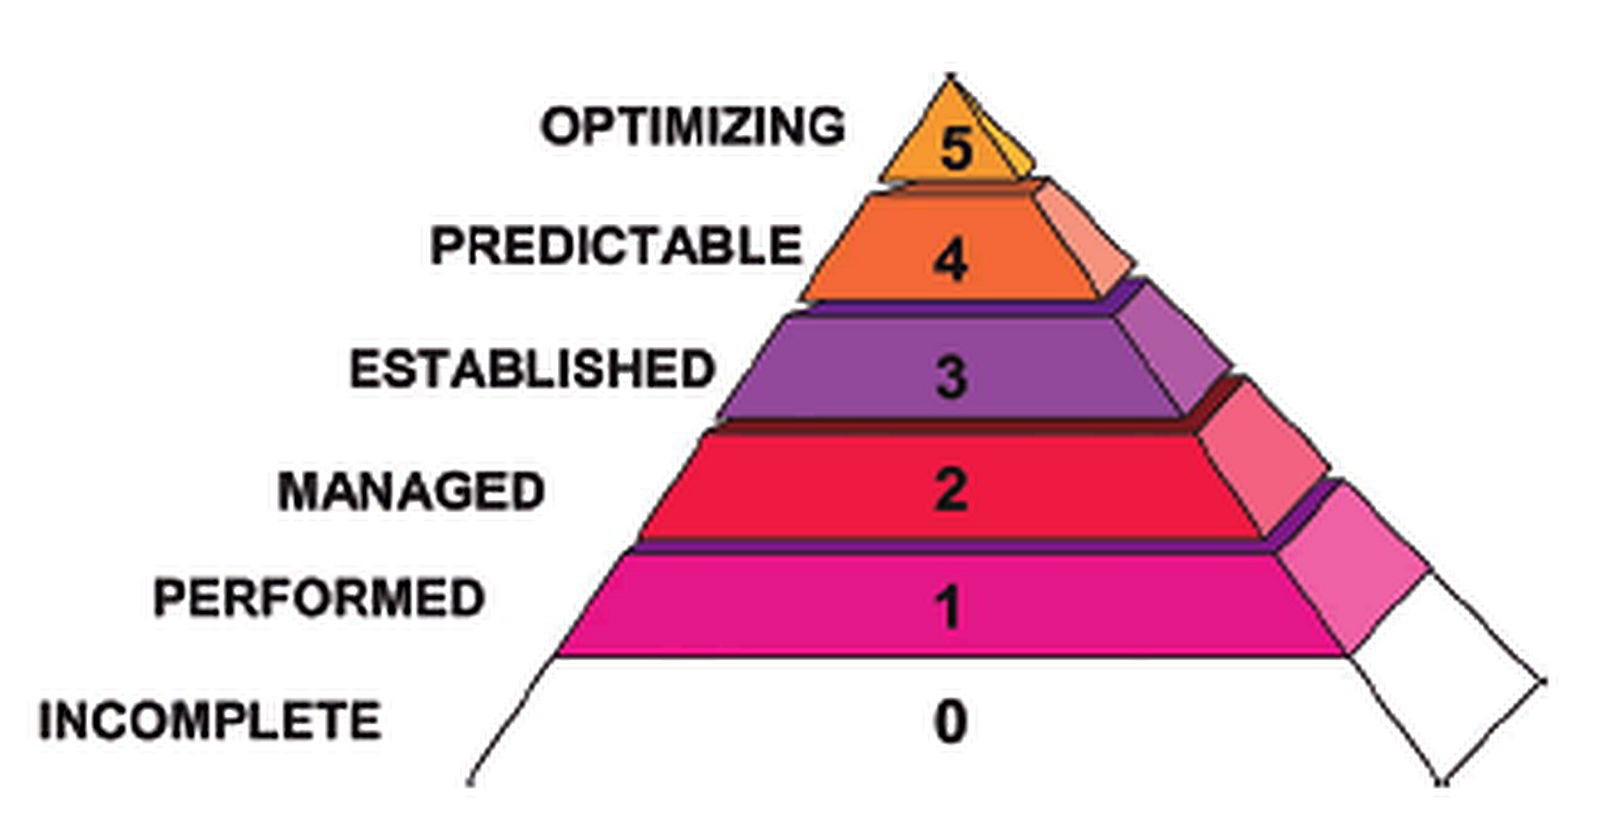
\includegraphics[scale=1.3]{img/Iso15504.jpg}
    \captionof{figure}{Standar ISO/IEC 15504 \\}
  \end{center}



  \begin{itemize}
  \item \textbf{Livello 0 - Incomplete process}\\
    Il processo non è implementato o non riesce a raggiungere i suoi obiettivi
  \item \textbf{Livello 1 - Performed process}\\
    Il processo viene messo in atto e raggiunge i suoi scopi
  \item  \textbf{Livello 2 - Managed process}\\
    Il processo viene eseguito sulla base di obiettivi ben definiti
  \item  \textbf{Livello 3 - Established process}\\
    Il processo viene eseguito in base ai principi dell’ingegneria del software
  \item  \textbf{Livello 4 - Predictable process}\\
    Il processo è attuato all’interno di limiti ben definiti
  \item  \textbf{Livello 5 - Optimizing process}\\
    Il processo è predicibile ed è in grado di adattarsi per raggiungere obiettivi specifici e rilevanti
  \end{itemize}

  Per valutare il livello di maturità di un processo si utilizzano le
  metriche descritte nella sezione \emph{2.8.1}, in particolare lo
  schedule variance aiuta a capire quando un processo raggiunge uno
  stato accettbile se il valore subisce al massimo lievi oscillazioni
  da quanto previsto.





  \subsection{Ciclo di Deming -  PDCA}
  Il ciclo di Deming (o PDCA) è un approccio manageriale per il
  controllo e il
  miglioramento continuo dei processi e dei prodoti ed è
  parte integrante della gestione della qualità.
  Il ciclo di Deming è suddiviso in quattro fasi: \\



  %\FloatBarrier
  \begin{center}
    % \centering
    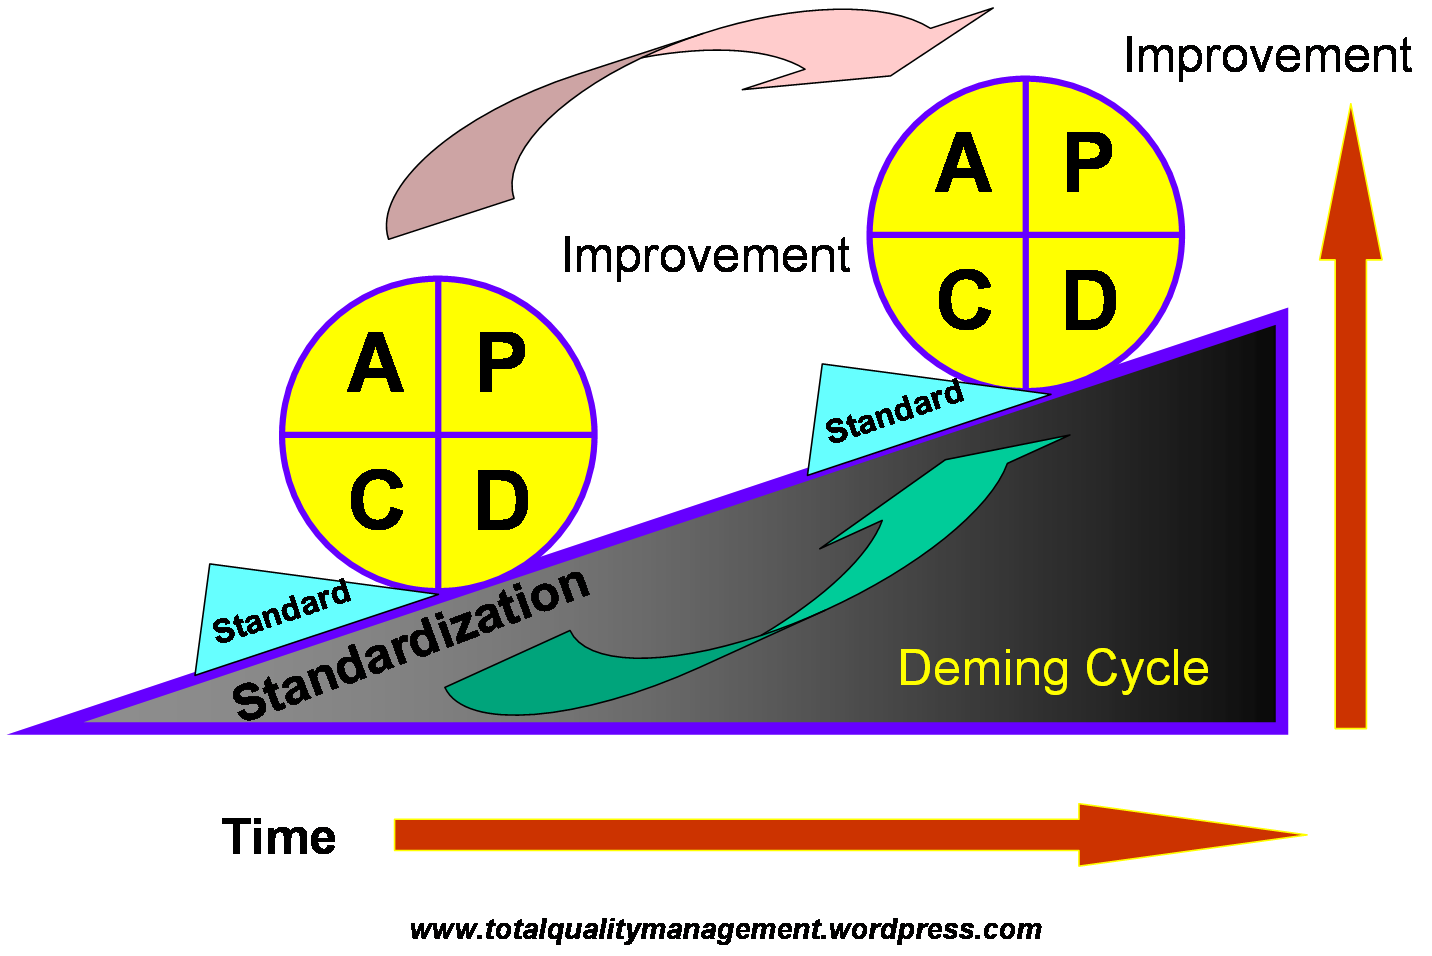
\includegraphics[scale=0.3]{img/deming.png}
    \captionof{figure}{Ciclo di Deming}
  \end{center}
  %\FloatBarrier



  \begin{itemize}
  \item  \textbf{Plan} - stabilire gli obiettivi e i processi necessari per
fornire risultati in accordo con i risultati attesi, attraverso la
creazione di attese di produzione, di completezza e accuratezza delle
specifiche scelte. Quando possibile, avvio su piccola scala, per
verificare i possibili effetti.

    %% \begin{itemize}
    %% \item Precisazione degli obiettivi del miglioramento da attuare
    %% \item Raccolta dei dati relativi al problema o processo
    %% \item Mappatura del processo utilizzando un diagramma di flusso od altro strumento utile
    %% \item Individuazione delle cause principali dei vincoli da rimuovere
    %% \item Determinazione degli interventi necessari per risolvere la situazione
    %% \item Determinazione dei risultati attesi
    %% \item Definizione delle responsabilità per la fase di attuazione
    %% \item Pianificazione delle azioni da svolgere
    %% \item Pianificazione delle risorse
    %% \item Determinazione delle metriche per misurare i miglioramenti o gli scostamenti da quanto previsto
    %% \end{itemize}

  \item  \textbf{Do} -  Esecuzione del programma, dapprima in contesti
    circoscritti. Attuare il piano, eseguire il processo, creare il
    prodotto. Raccogliere i dati per la creazione di grafici e analisi
    da destinare alla fase di "Check" e "Act". 
    %% \begin{itemize}
    %% \item I responsabili individuati mettono in pratica le azioni previste
    %% \item Ogni soluzione è implementata per un periodo di prova
    %% \item Viene verificata l’adeguatezza delle soluzioni adottate rispetto agli obiettivi attesi
    %% \item Vengono formati i dipendenti sulle nuove modalità operative a fronte delle soluzioni adottate
    %% \end{itemize}

  \item  \textbf{Check} - Test e controllo, studio e raccolta dei
    risultati e dei riscontri. Studiare i risultati, misurati e
    raccolti nella fase del "Do" confrontandoli con i risultati
    attesi, obiettivi del "Plan", per verificarne le eventuali
    differenze. Cercare le deviazioni nell'attuazione del piano e
    focalizzarsi sulla sua adeguatezza e completezza per consentirne
    l'esecuzione. I grafici dei dati possono rendere questo molto più
    facile, in quanto è possibile vedere le tendenze di più cicli
    PDCA, convertendo i dati raccolti in informazioni. L'informazione
    è utile per realizzare il passo successivo : "Act".

  \item  \textbf{Act} - Azione per rendere definitivo e/o migliorare
    il processo (estendere quanto testato dapprima in contesti
    circoscritti all'intera organizzazione). Richiede azioni
    correttive sulle differenze significative tra i risultati
    effettivi e previsti. Analizza le differenze per determinarne le
    cause e dove applicare le modifiche per ottenere il miglioramento
    del processo o del prodotto. Quando un procedimento, attraverso
    questi quattro passaggi, non comporta la necessità di migliorare
    la portata a cui è applicato, il ciclo PDCA può essere raffinato
    per pianificare e migliorare con maggiore dettaglio la successiva
    iterazione, oppure l'attenzione deve essere posta in una diversa
    fase del processo. 

    %% \begin{itemize}
    %% \item Standardizzare il miglioramento ottenuto applicandolo in via definitiva
    %% \item Individuare eventuali esigenze di formazione del personale per rendere operative le soluzioni adottate
    %% \item Continuare a monitorare la situazione ripetendo il ciclo più volte fino a raggiungere i miglioramenti desiderati
    %% \item Individuare altre opportunità di miglioramento
    %% \end{itemize}
  \end{itemize}





















  \subsection{Standard ISO/IEC 9126}

  Aderendo a questo standard il team si impegna a garantire nel prodotto
  le seguenti qualità (definite con relativa metrica, misura e
  strumenti di controllo): \\


  \begin{center}
    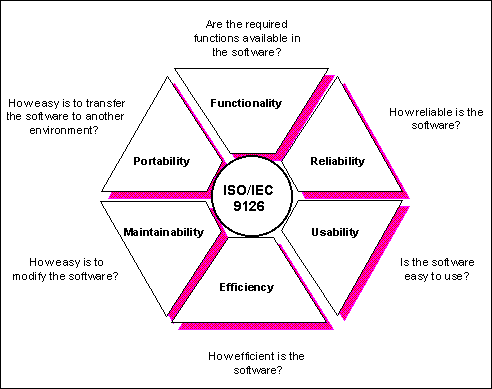
\includegraphics[scale=0.5]{img/9126s.png}
    \captionof{figure}{Standar ISO/IEC 9126}
  \end{center}




  \begin{enumerate}
  \item \textbf{Funzionalità}: il sistema prodotto deve garantire tutte
    le funzionalità indicate nel documento \emph{Analisi dei Requisiti
      vxxx} L'implementazione dei requisiti deve essere più completa
    possibile

    \begin{itemize}
    \item \textbf{Misura}: l’unità di misura usata sarà la quantità di requisiti mappati sulle componenti del sistema create e funzionanti
    \item \textbf{Metrica}: la sufficienza è stabilita nel soddisfacimento di tutti i requisiti obbligatori
    \item \textbf{Strumenti}: per soddisfare questa qualità il sistema deve superare tutti i test previsti.
      Per informazioni dettagliate sugli strumenti si veda  \emph{Norme di Progetto vxxx}
    \end{itemize}

  \item \textbf{Affidabilità}: il sistema deve dimostrarsi il più possibile robusto e di facile ripristino in caso di errori

    \begin{itemize}
    \item \textbf{Misura}: l’unità di misura utilizzata sarà la quantità di esecuzioni del sistema andate a buon fine
    \item \textbf{Metrica}: le esecuzioni dovranno spaziare il più
      possibile sulle varie parti del codice
    \item \textbf{Strumenti}: si vedano le metriche adottate per la
      copertura a %%%%%%%%%%%%%%%%%%%%%%%%%%%%%%%METRICHE
    \end{itemize}

  \item \textbf{Usabilità}: il sistema prodotto deve risultare di facile
    utilizzo per la classe di utenti a cui è destinato. Tale sistema
    deve essere facilmente apprendibile e allo stesso tempo deve
    soddisfare tutte le necessità dell’utente.
    \begin{itemize}
    \item \textbf{Misura}: l’unità di misura usata sarà una valutazione soggettiva dell’usabilità. Questo è dovuto all’inesistenza di una metrica oggettiva adatta allo scopo
    \item \textbf{Metrica}:  non esiste una metrica adeguata che determinerà la sufficienza su questa qualità
    \item \textbf{Strumenti}: si vedano le  \emph{Norme di Progetto vxxx}
    \end{itemize}

  \item \textbf{Efficienza}: il sistema deve fornire tutte le funzionalità nel più breve tempo possibile,
    riducendo al minimo l’utilizzo di risorse
    \begin{itemize}
    \item \textbf{Misura}: il tempo che lo sviluppatore impiegherà per la creazione di una bolla interattiva
    \item \textbf{Metrica}: non è possibile definire una soglia oggettiva di sufficienza perché non è possibile valutare ogni possibile casistica di utilizzo
    \item \textbf{Strumenti}: si vedano le  \emph{Norme di Progetto vxxx}
    \end{itemize}

  \item \textbf{Manutenibilità}: il sistema deve essere comprensibile ed estensibile in modo facile e verificabile
    \begin{itemize}
    \item \textbf{Misura}: le metriche sul codice descritte nella sezione \emph{2.8.2}
      costituiscono l'unità di misura
    \item \textbf{Metrica}: il software avrà le caratteristiche di manutenibilità descritte. Questo sarà possibile se il prodotto avrà la sufficienza in tutte le metriche
    \item \textbf{Strumenti}: si vedano le  \emph{Norme di Progetto vxxx}
    \end{itemize}

  \item \textbf{Portabilità}: il sistema deve essere il più portabile possibile, in particolare dentro a Rocket.chat
    \begin{itemize}
    \item \textbf{Misura}: il front end deve rispettare gli standard W3C
    \item \textbf{Metrica}: il software avrà le caratteristiche di
      portabilità descritte. Questo sarà possibile se il prodotto
      avrà la sufficienza in tutte le metriche, descritte nella sezione \emph{2.8.2}
    \item \textbf{Strumenti}: si vedano le \emph{Norme del Progetto vxxx}
    \end{itemize}
  \end{enumerate}




  \section{Resoconto delle attività di verifica}

  \subsection{Revisione dei Requisiti}

  L’attività di verifica svolta dai  \emph{Verificatori}  è avvenuta come determinato dal \emph{Piano di Progetto
    vxxx} al termine della stesura di ogni documento previsto. La verifica svolta sui documenti e
  sui processi è avvenuta seguendo le indicazioni delle  \emph{Norme di Progetto vxxx}  e misurando le
  metriche indicate nella sezione \emph{2.8.2}

  \subsubsection{Verifiche sui Processi}

  In questo periodo è stata svolta un' attività di walkthrough non avendo gli elementi
  per effettuare l'attività di inspection. Nella verifica dei
  documenti sono stati riscontrati soprattutto errori grammaticali e
  di battitura dovuti a disattenzioni durante la stesura. 

  \subsubsection{Documenti}
  Vengono qui riportati i valori dell’indice Gulpease per ogni documento durante l’analisi e relativo
  esito basato sui range stabiliti nella sezione \emph{2.8.2}
  \begin{center}
    \begin{tabular}{|c|c|c|}
      \hline
      \textbf{Documento} & \textbf{Valore indice} & \textbf{Esito} \\
      \hline
      \emph{Analisi dei Requisiti v1.0.0}  & 70 & superato \\
      % \hline
      %  \emph{Glossario v1.0.0}  & n & superato \\
      \hline
      \emph{Norme di Progetto v1.1.0}   & 58  & superato \\
      \hline
      \emph{Piano di Progetto v1.1.0}   & 65 & superato \\
      \hline
      \emph{Piano di Qualifica v1.0.0}   & 65 & superato \\
      \hline
      \emph{Studio di Fattibilità v1.0.0}  & 67 & superato \\
      \hline
    \end{tabular}
    \captionof{table}{Tabella risultati test Gulpease}
  \end{center}



  \subsection{Revisione di Progettazione}
  In questo periodo (antecedente la consegna di tale revisione) sono stati verificati i documenti ed i processi.

  \begin{itemize}
  \item Sono stati verificati i documenti applicando la procedura descritta nel documento \emph{Norme di progetto vxxx}
  \item \'E stata applicata \emph{l'analisi statica} secondo i criteri e le modalità indicata alla sezione \emph{2.7.1}.
 % \item Si è applicato il ciclo PDCA per rendere più efficiente ed efficace il processo di verifica.
  \item Si sono calcolate per i documenti le metriche descritte nella sezione \emph{2.8}.
  \item Il tracciamento (requisiti - componenti) è stato effettuato tramite un database MySQL creato ad uso interno.
  \item L’avanzamento dei processi è stato controllato e verificato secondo le metodiche descritte nelle \emph{Norme di Progetto vxxx}.

  \end{itemize}
  \subsubsection{Verifiche sui processi}

  Vengono qui riportati gli esiti delle verifiche sui processi produttivi.\\


  \textbf{Budget Variance / Schedule Variance}

  \begin{center}
    \begin{tabular}{|c|c|c|}

      \hline
      \textbf{Attività} & \textbf{SV} & \textbf{BV} \\
      \hline
      \emph{Analisi dei Requisiti 2.0.0} & 0€ & 0€ \\
      \hline
      \emph{Norme di Progetto 3.0.0} & +10€ & +70€ \\
      \hline
      \emph{Piano di Progetto 3.0.0} & 0€ & 0€ \\
      \hline
      \emph{Definizione di prodotto 1.0.0} & +25€ & -110€ \\
      \hline
      \emph{Piano di qualifica 3.0.0} & -10€ & 0€ \\
      \hline
      \emph{Glossario 2.0.0} & 0€ & 0€ \\
      \hline
    \end{tabular}
    \captionof{table}{Tabella risultati Budget Variance / Schedule Variance}
  \end{center}

  Complessivamente nel periodo di Revisione di Progettazione vengono misurate:
  \begin{itemize}
  \item Schedule Variance = 25€
  \item Budget Variance = -40€
  \end{itemize}

  Da valori di tali indici possiamo dedurre che:
  \begin{itemize}
  \item La data di fine della Revisione di Progettazione si è dimostrata essere un
    giorno prima di quella pianificata nel Piano di Progetto v3.0.0 .
    %% Aumentando il numero di ore di lavoro giornaliere ed utilizzando tutti gli slack
    %% inseriti durante la pianificazione il gruppo ha compresso i tempi con conseguente
    %% SV positivo;
  \item  Il limite inferiore di accettabilità del Budget Variance è pari a -436€.
    Il valore ottenuto risulta essere quindi accettabile. 
    %% Come già precisato, il
    %% gruppo per portare a termine gli obbiettivi entro le date imposte
    %% ha aumentato il numero di ore di lavoro giornaliere. 
    %% Questo ha quindi causato un aumento del BV in quanto le ore
    %% complessive di 
    %% lavoro sono state vicine a quelle preventivate, ma il periodo di lavoro è stato
    %% compresso.
  \end{itemize}


  \subsubsection{Verifica dei Documenti}
  Vengono qui riportati i valori dell’indice Gulpease per ogni documento durante l’analisi e relativo
  esito basato sui range stabiliti nella sezione \emph{2.8.2}
  \begin{center}
    \begin{tabular}{|c|c|c|}
      \hline
      \textbf{Documento} & \textbf{Valore indice} & \textbf{Esito} \\
      \hline
      \emph{Analisi dei Requisiti 2.0.0}  & 60.1 & superato \\
      \hline
      \emph{Norme di Progetto 3.0.0}   & 56.4  & superato \\
      \hline
      \emph{Piano di Progetto 3.0.0}   & 67.5 & superato \\
      \hline
      \emph{Piano di Qualifica 3.0.0}   & 61.4 & superato \\
      \hline
      \emph{Definizione di Prodotto 1.0.0}  & 76.9 & superato \\
      \hline
    \end{tabular}
    \captionof{table}{Tabella risultati test Gulpease}
  \end{center}
